% !TEX encoding = UTF-8 Unicode
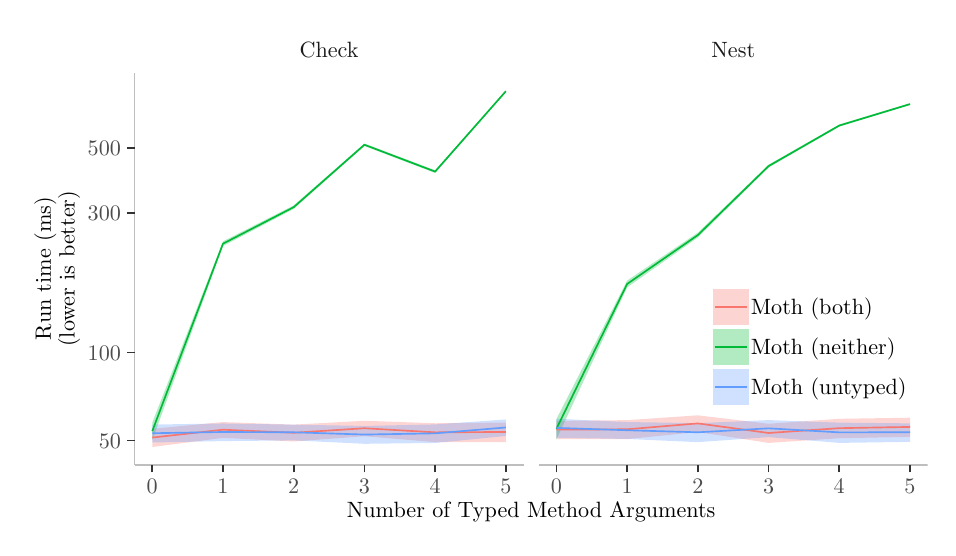
\begin{tikzpicture}[x=1pt,y=1pt]
\definecolor{fillColor}{RGB}{255,255,255}
\path[use as bounding box,fill=fillColor,fill opacity=0.00] (0,0) rectangle (325.21,180.67);
\begin{scope}
\path[clip] ( 38.64, 22.70) rectangle (179.18,164.42);
\definecolor{fillColor}{RGB}{248,118,109}

\path[fill=fillColor,fill opacity=0.30] ( 45.02, 35.72) --
	( 70.58, 38.15) --
	( 96.13, 37.23) --
	(121.68, 38.62) --
	(147.23, 37.72) --
	(172.79, 37.99) --
	(172.79, 30.90) --
	(147.23, 30.91) --
	(121.68, 33.04) --
	( 96.13, 31.15) --
	( 70.58, 32.44) --
	( 45.02, 29.14) --
	cycle;
\definecolor{fillColor}{RGB}{0,186,56}

\path[fill=fillColor,fill opacity=0.30] ( 45.02, 37.93) --
	( 70.58,103.45) --
	( 96.13,116.45) --
	(121.68,138.80) --
	(147.23,129.15) --
	(172.79,157.98) --
	(172.79,157.43) --
	(147.23,128.17) --
	(121.68,137.92) --
	( 96.13,115.16) --
	( 70.58,101.75) --
	( 45.02, 31.59) --
	cycle;
\definecolor{fillColor}{RGB}{97,156,255}

\path[fill=fillColor,fill opacity=0.30] ( 45.02, 37.25) --
	( 70.58, 37.65) --
	( 96.13, 37.22) --
	(121.68, 36.75) --
	(147.23, 37.31) --
	(172.79, 39.10) --
	(172.79, 33.13) --
	(147.23, 30.60) --
	(121.68, 30.30) --
	( 96.13, 31.53) --
	( 70.58, 31.28) --
	( 45.02, 30.77) --
	cycle;
\definecolor{drawColor}{RGB}{248,118,109}

\path[draw=drawColor,line width= 0.6pt,line join=round] ( 45.02, 32.55) --
	( 70.58, 35.39) --
	( 96.13, 34.29) --
	(121.68, 35.92) --
	(147.23, 34.44) --
	(172.79, 34.58);
\definecolor{drawColor}{RGB}{0,186,56}

\path[draw=drawColor,line width= 0.6pt,line join=round] ( 45.02, 34.87) --
	( 70.58,102.61) --
	( 96.13,115.81) --
	(121.68,138.36) --
	(147.23,128.66) --
	(172.79,157.70);
\definecolor{drawColor}{RGB}{97,156,255}

\path[draw=drawColor,line width= 0.6pt,line join=round] ( 45.02, 34.12) --
	( 70.58, 34.57) --
	( 96.13, 34.46) --
	(121.68, 33.64) --
	(147.23, 34.08) --
	(172.79, 36.21);
\end{scope}
\begin{scope}
\path[clip] (184.68, 22.70) rectangle (325.21,164.42);
\definecolor{fillColor}{RGB}{248,118,109}

\path[fill=fillColor,fill opacity=0.30] (191.06, 38.57) --
	(216.62, 38.85) --
	(242.17, 40.59) --
	(267.72, 37.54) --
	(293.27, 39.33) --
	(318.83, 39.73) --
	(318.83, 32.80) --
	(293.27, 32.31) --
	(267.72, 30.63) --
	(242.17, 34.55) --
	(216.62, 32.00) --
	(191.06, 32.02) --
	cycle;
\definecolor{fillColor}{RGB}{0,186,56}

\path[fill=fillColor,fill opacity=0.30] (191.06, 39.25) --
	(216.62, 89.28) --
	(242.17,106.60) --
	(267.72,131.16) --
	(293.27,145.67) --
	(318.83,153.37) --
	(318.83,152.72) --
	(293.27,144.92) --
	(267.72,130.13) --
	(242.17,104.84) --
	(216.62, 86.82) --
	(191.06, 31.90) --
	cycle;
\definecolor{fillColor}{RGB}{97,156,255}

\path[fill=fillColor,fill opacity=0.30] (191.06, 39.35) --
	(216.62, 38.16) --
	(242.17, 37.77) --
	(267.72, 38.87) --
	(293.27, 37.95) --
	(318.83, 37.69) --
	(318.83, 31.00) --
	(293.27, 30.63) --
	(267.72, 32.71) --
	(242.17, 30.90) --
	(216.62, 32.05) --
	(191.06, 32.50) --
	cycle;
\definecolor{drawColor}{RGB}{248,118,109}

\path[draw=drawColor,line width= 0.6pt,line join=round] (191.06, 35.41) --
	(216.62, 35.55) --
	(242.17, 37.67) --
	(267.72, 34.21) --
	(293.27, 35.95) --
	(318.83, 36.40);
\definecolor{drawColor}{RGB}{0,186,56}

\path[draw=drawColor,line width= 0.6pt,line join=round] (191.06, 35.72) --
	(216.62, 88.06) --
	(242.17,105.73) --
	(267.72,130.65) --
	(293.27,145.30) --
	(318.83,153.05);
\definecolor{drawColor}{RGB}{97,156,255}

\path[draw=drawColor,line width= 0.6pt,line join=round] (191.06, 36.05) --
	(216.62, 35.20) --
	(242.17, 34.46) --
	(267.72, 35.89) --
	(293.27, 34.43) --
	(318.83, 34.47);
\end{scope}
\begin{scope}
\path[clip] ( 38.64,164.42) rectangle (179.18,180.67);
\definecolor{drawColor}{gray}{0.10}

\node[text=drawColor,anchor=base,inner sep=0pt, outer sep=0pt, scale=  0.80] at (108.91,169.79) {Check};
\end{scope}
\begin{scope}
\path[clip] (184.68,164.42) rectangle (325.21,180.67);
\definecolor{drawColor}{gray}{0.10}

\node[text=drawColor,anchor=base,inner sep=0pt, outer sep=0pt, scale=  0.80] at (254.95,169.79) {Nest};
\end{scope}
\begin{scope}
\path[clip] (  0.00,  0.00) rectangle (325.21,180.67);
\definecolor{drawColor}{RGB}{190,190,190}

\path[draw=drawColor,line width= 0.6pt,line join=round] ( 38.64, 22.70) --
	(179.18, 22.70);
\end{scope}
\begin{scope}
\path[clip] (  0.00,  0.00) rectangle (325.21,180.67);
\definecolor{drawColor}{gray}{0.20}

\path[draw=drawColor,line width= 0.6pt,line join=round] ( 45.02, 19.95) --
	( 45.02, 22.70);

\path[draw=drawColor,line width= 0.6pt,line join=round] ( 70.58, 19.95) --
	( 70.58, 22.70);

\path[draw=drawColor,line width= 0.6pt,line join=round] ( 96.13, 19.95) --
	( 96.13, 22.70);

\path[draw=drawColor,line width= 0.6pt,line join=round] (121.68, 19.95) --
	(121.68, 22.70);

\path[draw=drawColor,line width= 0.6pt,line join=round] (147.23, 19.95) --
	(147.23, 22.70);

\path[draw=drawColor,line width= 0.6pt,line join=round] (172.79, 19.95) --
	(172.79, 22.70);
\end{scope}
\begin{scope}
\path[clip] (  0.00,  0.00) rectangle (325.21,180.67);
\definecolor{drawColor}{gray}{0.30}

\node[text=drawColor,anchor=base,inner sep=0pt, outer sep=0pt, scale=  0.80] at ( 45.02, 12.24) {0};

\node[text=drawColor,anchor=base,inner sep=0pt, outer sep=0pt, scale=  0.80] at ( 70.58, 12.24) {1};

\node[text=drawColor,anchor=base,inner sep=0pt, outer sep=0pt, scale=  0.80] at ( 96.13, 12.24) {2};

\node[text=drawColor,anchor=base,inner sep=0pt, outer sep=0pt, scale=  0.80] at (121.68, 12.24) {3};

\node[text=drawColor,anchor=base,inner sep=0pt, outer sep=0pt, scale=  0.80] at (147.23, 12.24) {4};

\node[text=drawColor,anchor=base,inner sep=0pt, outer sep=0pt, scale=  0.80] at (172.79, 12.24) {5};
\end{scope}
\begin{scope}
\path[clip] (  0.00,  0.00) rectangle (325.21,180.67);
\definecolor{drawColor}{RGB}{190,190,190}

\path[draw=drawColor,line width= 0.6pt,line join=round] (184.68, 22.70) --
	(325.21, 22.70);
\end{scope}
\begin{scope}
\path[clip] (  0.00,  0.00) rectangle (325.21,180.67);
\definecolor{drawColor}{gray}{0.20}

\path[draw=drawColor,line width= 0.6pt,line join=round] (191.06, 19.95) --
	(191.06, 22.70);

\path[draw=drawColor,line width= 0.6pt,line join=round] (216.62, 19.95) --
	(216.62, 22.70);

\path[draw=drawColor,line width= 0.6pt,line join=round] (242.17, 19.95) --
	(242.17, 22.70);

\path[draw=drawColor,line width= 0.6pt,line join=round] (267.72, 19.95) --
	(267.72, 22.70);

\path[draw=drawColor,line width= 0.6pt,line join=round] (293.27, 19.95) --
	(293.27, 22.70);

\path[draw=drawColor,line width= 0.6pt,line join=round] (318.83, 19.95) --
	(318.83, 22.70);
\end{scope}
\begin{scope}
\path[clip] (  0.00,  0.00) rectangle (325.21,180.67);
\definecolor{drawColor}{gray}{0.30}

\node[text=drawColor,anchor=base,inner sep=0pt, outer sep=0pt, scale=  0.80] at (191.06, 12.24) {0};

\node[text=drawColor,anchor=base,inner sep=0pt, outer sep=0pt, scale=  0.80] at (216.62, 12.24) {1};

\node[text=drawColor,anchor=base,inner sep=0pt, outer sep=0pt, scale=  0.80] at (242.17, 12.24) {2};

\node[text=drawColor,anchor=base,inner sep=0pt, outer sep=0pt, scale=  0.80] at (267.72, 12.24) {3};

\node[text=drawColor,anchor=base,inner sep=0pt, outer sep=0pt, scale=  0.80] at (293.27, 12.24) {4};

\node[text=drawColor,anchor=base,inner sep=0pt, outer sep=0pt, scale=  0.80] at (318.83, 12.24) {5};
\end{scope}
\begin{scope}
\path[clip] (  0.00,  0.00) rectangle (325.21,180.67);
\definecolor{drawColor}{RGB}{190,190,190}

\path[draw=drawColor,line width= 0.6pt,line join=round] ( 38.64, 22.70) --
	( 38.64,164.42);
\end{scope}
\begin{scope}
\path[clip] (  0.00,  0.00) rectangle (325.21,180.67);
\definecolor{drawColor}{gray}{0.30}

\node[text=drawColor,anchor=base east,inner sep=0pt, outer sep=0pt, scale=  0.80] at ( 33.69, 28.69) {50};

\node[text=drawColor,anchor=base east,inner sep=0pt, outer sep=0pt, scale=  0.80] at ( 33.69, 60.54) {100};

\node[text=drawColor,anchor=base east,inner sep=0pt, outer sep=0pt, scale=  0.80] at ( 33.69,111.01) {300};

\node[text=drawColor,anchor=base east,inner sep=0pt, outer sep=0pt, scale=  0.80] at ( 33.69,134.48) {500};
\end{scope}
\begin{scope}
\path[clip] (  0.00,  0.00) rectangle (325.21,180.67);
\definecolor{drawColor}{gray}{0.20}

\path[draw=drawColor,line width= 0.6pt,line join=round] ( 35.89, 31.45) --
	( 38.64, 31.45);

\path[draw=drawColor,line width= 0.6pt,line join=round] ( 35.89, 63.29) --
	( 38.64, 63.29);

\path[draw=drawColor,line width= 0.6pt,line join=round] ( 35.89,113.76) --
	( 38.64,113.76);

\path[draw=drawColor,line width= 0.6pt,line join=round] ( 35.89,137.23) --
	( 38.64,137.23);
\end{scope}
\begin{scope}
\path[clip] (  0.00,  0.00) rectangle (325.21,180.67);
\definecolor{drawColor}{RGB}{0,0,0}

\node[text=drawColor,anchor=base,inner sep=0pt, outer sep=0pt, scale=  0.80] at (181.93,  3.82) {Number of Typed Method Arguments};
\end{scope}
\begin{scope}
\path[clip] (  0.00,  0.00) rectangle (325.21,180.67);
\definecolor{drawColor}{RGB}{0,0,0}

\node[text=drawColor,rotate= 90.00,anchor=base,inner sep=0pt, outer sep=0pt, scale=  0.80] at (  8.36, 93.56) {Run time (ms)};

\node[text=drawColor,rotate= 90.00,anchor=base,inner sep=0pt, outer sep=0pt, scale=  0.80] at ( 17.00, 93.56) {(lower is better)};
\end{scope}
\begin{scope}
\path[clip] (  0.00,  0.00) rectangle (325.21,180.67);
\definecolor{fillColor}{RGB}{255,255,255}

\path[fill=fillColor] (246.90, 72.45) rectangle (261.35, 86.90);
\end{scope}
\begin{scope}
\path[clip] (  0.00,  0.00) rectangle (325.21,180.67);
\definecolor{fillColor}{RGB}{248,118,109}

\path[fill=fillColor,fill opacity=0.30] (247.61, 73.16) rectangle (260.64, 86.19);
\end{scope}
\begin{scope}
\path[clip] (  0.00,  0.00) rectangle (325.21,180.67);
\definecolor{drawColor}{RGB}{248,118,109}

\path[draw=drawColor,line width= 0.6pt,line join=round] (248.34, 79.67) -- (259.91, 79.67);
\end{scope}
\begin{scope}
\path[clip] (  0.00,  0.00) rectangle (325.21,180.67);
\definecolor{fillColor}{RGB}{255,255,255}

\path[fill=fillColor] (246.90, 57.99) rectangle (261.35, 72.45);
\end{scope}
\begin{scope}
\path[clip] (  0.00,  0.00) rectangle (325.21,180.67);
\definecolor{fillColor}{RGB}{0,186,56}

\path[fill=fillColor,fill opacity=0.30] (247.61, 58.70) rectangle (260.64, 71.73);
\end{scope}
\begin{scope}
\path[clip] (  0.00,  0.00) rectangle (325.21,180.67);
\definecolor{drawColor}{RGB}{0,186,56}

\path[draw=drawColor,line width= 0.6pt,line join=round] (248.34, 65.22) -- (259.91, 65.22);
\end{scope}
\begin{scope}
\path[clip] (  0.00,  0.00) rectangle (325.21,180.67);
\definecolor{fillColor}{RGB}{255,255,255}

\path[fill=fillColor] (246.90, 43.54) rectangle (261.35, 57.99);
\end{scope}
\begin{scope}
\path[clip] (  0.00,  0.00) rectangle (325.21,180.67);
\definecolor{fillColor}{RGB}{97,156,255}

\path[fill=fillColor,fill opacity=0.30] (247.61, 44.25) rectangle (260.64, 57.28);
\end{scope}
\begin{scope}
\path[clip] (  0.00,  0.00) rectangle (325.21,180.67);
\definecolor{drawColor}{RGB}{97,156,255}

\path[draw=drawColor,line width= 0.6pt,line join=round] (248.34, 50.76) -- (259.91, 50.76);
\end{scope}
\begin{scope}
\path[clip] (  0.00,  0.00) rectangle (325.21,180.67);
\definecolor{drawColor}{RGB}{0,0,0}

\node[text=drawColor,anchor=base west,inner sep=0pt, outer sep=0pt, scale=  0.80] at (261.35, 76.92) {Moth (both)};
\end{scope}
\begin{scope}
\path[clip] (  0.00,  0.00) rectangle (325.21,180.67);
\definecolor{drawColor}{RGB}{0,0,0}

\node[text=drawColor,anchor=base west,inner sep=0pt, outer sep=0pt, scale=  0.80] at (261.35, 62.46) {Moth (neither)};
\end{scope}
\begin{scope}
\path[clip] (  0.00,  0.00) rectangle (325.21,180.67);
\definecolor{drawColor}{RGB}{0,0,0}

\node[text=drawColor,anchor=base west,inner sep=0pt, outer sep=0pt, scale=  0.80] at (261.35, 48.01) {Moth (untyped)};
\end{scope}
\end{tikzpicture}
